\section{Evaluation}
\label{evaluation}

In this section, we evaluate Spatial by comparing programmer productivity and the performance of generated designs to Xilinx's commercial HLS tool, SDAccel. We then evaluate the HyperMapper design tuning approach and demonstrate Spatial's advantages for portability across FPGAs and the Plasticine CGRA.

\subsection{FPGA Performance and Productivity}
We first evaluate the FPGA performance and productivity benefits of Spatial against SDAccel, a commercial C-based programming tool from Xilinx for creating high-performance accelerator designs. We use SDAccel in our study as it has similar performance and productivity goals as Spatial, supports the popular OpenCL programming model, and performs several optimizations related to loop pipelining, unrolling, and memory partitioning~\cite{sdaccel}. Baseline implementations of the benchmarks in Table~\ref{t:hls_comp} have been either obtained from a public SDAccel benchmark suite from Xilinx~\cite{sdaccelBench}, or written by hand. Each baseline has then been manually tuned by using appropriate HLS pragmas~\cite{hlsPragmaRef} to pick loop pipelining, unrolling, and array banking factors, and to enable dataflow optimizations. Design points for Spatial are chosen using the DSE flow described in Section~\ref{dse}.

We measure productivity by comparing number of lines of source code used to describe the FPGA kernel, excluding host code. We measure performance by comparing runtimes and FPGA resources utilized for each benchmark on a Xilinx Ultrascale+ VU9P board with a fabric clock of 125 MHz, hosted on an Amazon EC2 F1 instance. We generate FPGA bitstreams targeting the VU9P architecture for each benchmark using both Spatial and SDAccel, and obtain resource utilization data from the post place-and-route reports. We then run and verify both designs on the FPGA and measure the execution times on the board. CPU setup code and data transfer time between CPU and FPGA is excluded from runtime measurements for both tools.

Table~\ref{t:hls_comp} shows the input dataset sizes and the full comparison between lines of source code, resource utilization, and runtime of the benchmarks implemented in SDAccel and Spatial.
In terms of productivity, language constructs in Spatial like \texttt{\small{load}} and \texttt{\small{store}} for transferring dense sparse data from DRAM reduces code bloat and increases readability.
Furthermore, by implicitly
inferring parameters such as parallelization factors and loop initiation intervals, Spatial code is largely free of annotations and pragmas.

Spatial achieves speedups over SDAccel of $1.63\times$ and $1.33\times$ respectively on \emph{BlackScholes} and \emph{TPC-H Q6}. Both benchmarks
stream data from DRAM through a deeply pipelined datapath which is amenable to FPGA acceleration. Dataflow support in SDAccel using the DATAFLOW pragma~\cite{dataflowRef} and streaming support in Spatial allows both tools to efficiently accelerate such workloads. In \emph{K-Means}, coarse-grained pipelining support allows Spatial to achieve roughly the same performance as SDAccel using $1.5\times$ fewer BRAMs.
Specialized DRAM scatter/gather support enables Spatial to achieve a $3.48\times$ speedup on \emph{PageRank}.

We see speedups of $8.48\times$, $1.37\times$, and $14.15\times$ for compute-heavy workloads \emph{GDA}, \emph{GEMM}, and \emph{SW}, respectively. The baseline for \emph{SW} is implemented by Xilinx as a systolic array, while the Spatial implementation uses nested controllers. \emph{GEMM} and \emph{GDA} contain opportunities for coarse-grained pipelining that are exploited within Spatial. 
GDA, for example, contains an outer product operation, during which the data in the same buffer is repeatedly accessed and reused. While this operation can be pipelined with a preceding loop producing the array, SDAccel's DATAFLOW pragma does not support such access patterns that involve reuse. As a result, SDAccel requires larger array partitioning and loop unrolling factors to offset the performance impact, at the expense of consuming more FPGA BRAM.
In addition, nested controllers in \emph{GEMM}
can be parallelized and pipelined independently in Spatial, while SDAccel automatically unrolls all inner loops if an outer loop is parallelized. Spatial can therefore explore
design points that cannot be easily expressed in SDAccel. Finally, as the Spatial compiler performs analyses on a parameterized IR, the compiler can reason about larger parallelization factors without expanding the IR graph.
SDAccel unrolls the graph as a preprocessing step, hence creating larger graphs when unrolling and array partitioning factors are large.
This has a significant impact on the compiler's memory footprint and compilation times, making better designs difficult or impossible to find.

Spatial provides a productive platform to program FPGAs, with a 42\% reduction in lines of code compared to SDAccel averaged across all benchmarks. On the studied benchmarks, Spatial achieves a geometric mean speedup of $2.9\times$ compared to an industrial HLS tool.


\subsection{Design Space Exploration}

We evaluate the accuracy of the estimations described in Section~\ref{sec:modeling}. We use our models to
study the space of designs on benchmarks from the data analytics,
machine learning, and financial analytics domains. We then evaluate the speed of our design
space exploration against a commercial high-level synthesis tool.
Finally, we evaluate the performance of our
Pareto-optimal points by comparing the execution times with an optimized multicore CPU implementation on a server-grade processor.
\subsection{Experimental Setup}

\begin{table}
\centering\footnotesize
\begin{tabular}{lm{3.6cm}m{2cm}}
\toprule

{\bf Benchmark} & {\bf Description} & {\bf Dataset Size} \\ \midrule
dotproduct   & Vector dot product & 187,200,000\\ \midrule
outerproduct & Vector outer product & $38,400$ $38,400$ \\ \midrule
%sumrows & Matrix summation through rows & $1M \times 1M$\\ \midrule
gemm         & Tiled matrix multiplication & $1536 \times 1536$\\ \midrule
tpchq6       & TPC-H Query 6 & N=18,720,000 \\ \midrule
blackscholes & Black-Scholes-Merton model & N=9,995,328 \\ \midrule
gda         & Gaussian discriminant analysis & R=360,000 D=96 \\ \midrule
kmeans & $k$-Means clustering & \#points=960,000, k=8, dim=384 \\ \midrule
%knn & $k$-Nearest neighbors algorithm & \#points=1M, \#test=960, k=64, dim=96 \\ \bottomrule
%knn & k Nearest Neighbors & MultiFold, Map, GroupByFold \\ \bottomrule
\end{tabular}
\caption{Evaluation benchmarks.}
\label{t:benchmarks}
\end{table}

Table~\ref{t:benchmarks} lists the benchmarks we use in our evaluation along with the corresponding
input dataset sizes used. \emph{Dotproduct}, \emph{outerprod}, and \emph{gemm} are common
linear algebra kernels. \emph{Tpchq6} is a data analytics application that streams through a collection
of records and performs a reduction on records filtered by a condition. \emph{BlackScholes} is
a financial analytics application that implements Black-Scholes option pricing. \emph{Gda}
and \emph{kmeans}
%and \emph{k}-nearest neighbors
are commonly used machine learning kernels used for data classification and clustering, respectively.
All benchmarks operate on single-precision floating point numbers,
except in certain cases where the benchmark requires integer or boolean values as inputs.
For the purposes of this paper, all benchmarks were written in DHDL by hand but are equivalent to what
could be generated automatically from higher level DSLs.

We implement the DHDL compiler framework in Scala. The DHDL compiler generates hardware by emitting
MaxJ, which is a low-level Java-based hardware generation language. Each generated design is synthesized
and run on an Altera 28nm Stratix V FPGA on a Max4 MAIA board at a fabric clock frequency of 150MHz.
The MAIA board interfaces with an Intel CPU
via PCIe. The board has 48GB of dedicated off-chip DDR3 DRAM with a peak bandwidth of 76.8GB/s. In practice,
our maximum memory bandwidth is 37.5 GB/s, as our on-chip memory clock is limited to 400MHz.
We leverage Maxeler's runtime to manage communication and data movement between the host CPU and
the MAIA board.
Execution time is measured starting
from when the FPGA design is started (after input has been copied to FPGA DRAM) and stopped after
the design finishes execution (before output is copied to CPU DRAM). We report execution time as the
average of 20 runs to eliminate noise from design initialization time and off-chip memory latencies.
The FPGA resource utilization
numbers reported are from the post place-and-route report generated by Altera's logic synthesis tools.

\subsection{Evaluation of estimator}

\begin{table}
\centering\footnotesize
\begin{tabular}{lcccc}
\toprule

{\bf Benchmark} & {\bf ALMs} & {\bf DSPs} & {\bf BRAM} & {\bf Runtime} \\ \midrule
dotproduct      & 1.7\%      & 0.0\%      & 13.1\%      & 2.8\%  \\ \midrule
outerproduct    & 4.4\%      & 29.7\%     & 12.8\%      & 1.3\%  \\ \midrule
gemm            & 12.7\%     & 11.4\%     & 17.4\%      & 18.4\% \\ \midrule
tpchq6          & 2.3\%      & 0.0\%      & 5.4\%       & 3.1\%  \\ \midrule
blackscholes    & 5.3\%      & 5.3\%      & 7.0\%       & 3.4\%  \\ \midrule
gda             & 5.2\%      & 6.2\%      & 8.4\%       & 6.7\%  \\ \midrule
kmeans          & 2.0\%      & 0.0\%      & 21.9\%      & 7.0\%  \\ \midrule \midrule

Average         & 4.8\%      & 7.5\%     & 12.3\%      & 6.1\%   \\ \bottomrule
\end{tabular}
\caption{Average absolute error for resource usage and runtime.}
\label{t:errors}
\end{table}

We first evaluate the absolute accuracy of our modeling approach. We select five Pareto points generated from our design space exploration for each of our benchmarks. We then generate and synthesize hardware for each design and run it on the FPGA. We compare our area estimates to post place-and-route reports generated by Altera's toolchain. We then run the design on the FPGA and compare the estimated runtime to observed runtime. Note that runtime includes off-chip memory accesses from the FPGA to its DRAM. Table~\ref{t:errors} summarizes the errors averaged across all selected Pareto points for each benchmark.

Our area estimates have an average error of 4.8\% for ALMs, 7.5\% for DSPs, and 12.3\% for BRAMs, while our runtime estimation error averages 6.1\%.
Our highest error occurs in predicting DSPs for \emph{outerprod}, where we over-predict by 29.7\% DSP usage on average.
However, we found that errors above 10\% for DSP usage only occur for designs which use less than 2\% of the total DSPs available on the device.
As our benchmarks are limited by other resources (typically ALMs or BRAM), the relative error for DSPs is more sensitive
to low-level fluctuations and noise. We observe that our DSP estimates preserve absolute ordering of resource utilization. Hence, this error does not
affect the quality of the designs found during design space exploration, and improves with increased resource utilization.

Of our estimated metrics, BRAM estimates have the highest average error over all benchmarks. These errors are primarily from block RAM duplication done by the placement and routing tool. In designing our models, we found that BRAM duplication is inherently noisy, as more complex machine learning models failed to achieve better estimates than a simple linear fit. Our linear model provides a rough estimate of design complexity and routing requirements, but it does not provide a complete picture for when and how often the synthesis tool will decide to duplicate BRAMs. However, like DSPs, we find that our BRAM estimates track actual usage and preserve ordering across designs, making it usable for design space exploration and relative design comparisons.

\emph{GEMM} has the highest overall error of any benchmark. We found that this is due to low-level hardware optimizations like floating point multiply-add fusion, fusion of floating point reduction trees, and BRAM coalescing that Maxeler's compiler performs automatically and that we use heuristics to predict. Since we do not have explicit control over these optimizations, it is possible to mispredict when they will occur. The \emph{gemm} benchmark is exceptionally sensitive to these errors. However, as with the other errors, we found that this error does not detract from the model's ability to guide design space exploration as long as the possibility of this error is accounted for.


\begin{figure*}[!htbp]
\centering
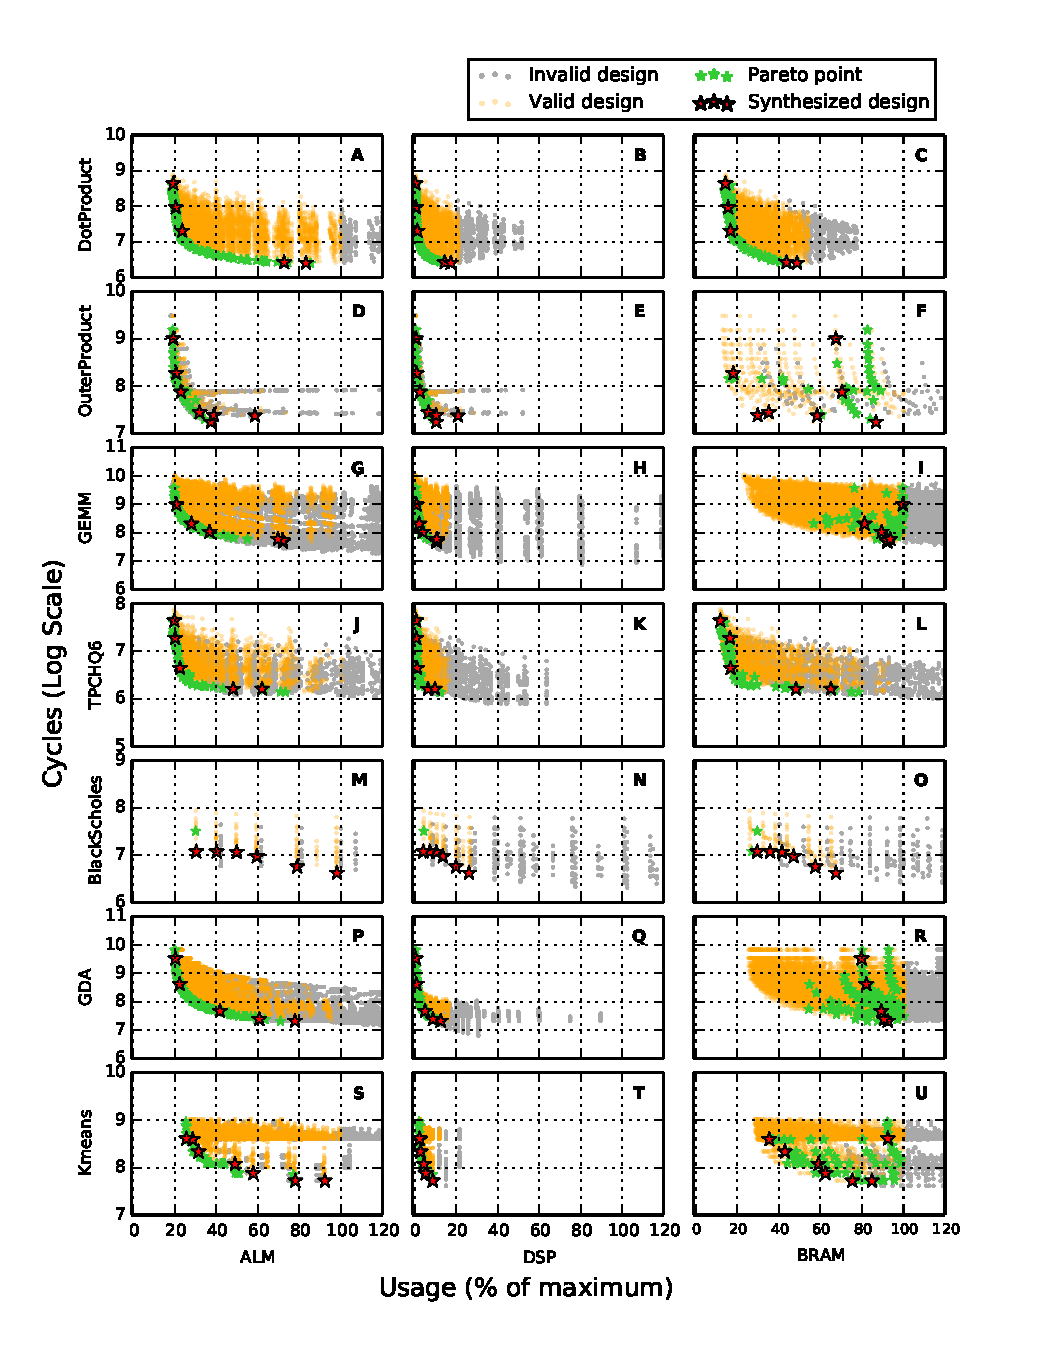
\includegraphics[width=0.95\textwidth]{figs/tradeoff.pdf}
\caption{Results of design space exploration. Horizontal axis shows estimated ALM, DSP, and BRAM usages. Vertical axis shows runtime in cycles, given in log scale (base 10).}
\label{fig:dse}
\end{figure*}

%\begin{figure*}[ht]
\subsection{Design space exploration}
\subsubsection{Pareto-optimality analysis}
In this section we show the Pareto-optimal curves of each benchmark derived from estimators.
%
Figure~\ref{fig:dse} shows the design space scatter plots for all benchmarks in
Table~\ref{t:benchmarks}. A design point is considered
invalid if its resource requirement for at least one type of resource exceeds the maximum
available amount on the target device. Pareto-optimal designs along the dimensions of execution time
and ALM utilization are highlighted for each benchmark through all three resource plots.
We now analyze each benchmark in detail.

\textbf{Dot product} (Figure~\ref{fig:dse} A,B,C) is a memory-bound benchmark. Peak execution
time is reached by balancing tile loads and computation. Inner and outer loop parallelization allows us to
quickly reach close to the input bandwidth. Runtimes of designs with \emph{MetaPipe}s then slowly decrease as parallelization
increases once the dominant stage becomes the dot product reduction tree. In \emph{dotproduct}, designs with \emph{MetaPipe} consume less resources than those with \emph{Sequential} for the same performance. \emph{Sequential}s require larger tile sizes and more parallelism to match \emph{MetaPipe} performance.

\textbf{Outer product} (Figure~\ref{fig:dse} D,E,F) represents both a BRAM and memory bound benchmark. For $2N$ inputs,
the total BRAM requirement is $2N + N^2$ to store the input and output tiles, meaning the BRAM requirement
increases quadratically with increases in input tile size. The highest performing designs for outer product do not use
\emph{MetaPipes} to overlap loading and storing of tiles. This is because the overhead due to main memory contention from overlapping
tile loads and stores turns out to be higher than the cost of executing each stage sequentially.

\textbf{GEMM} (Figure~\ref{fig:dse} G,H,I) contains a lot of temporal and spatial locality. From Figure~\ref{fig:dse}(I), Pareto-optimal designs for \emph{gemm}
occupy almost all BRAM resources on the board. Intuitively, this is  because good designs for \emph{gemm}
maximize locality by retaining large, two dimensional chunks of data in on-chip memory.
%However, as seen in Figure~\ref{fig:dse}(G), \emph{gemm} is also limited by the
%number of ALMs due to the large number of floating point operations being done in parallel.

\textbf{TPC-H Q6} (Figure~\ref{fig:dse} J,K,L) exhibits behavior typical of memory intensive applications. Performance reaches a maximum threshold
with increased tile size because of overlapping memory access and compute.

\textbf{BlackScholes} (Figure~\ref{fig:dse} M,N,O) streams through multiple large arrays and performs complex floating point computations
on the input data. Points along the same vertical bar in Figure~\ref{fig:dse}(M) share the same inner loop parallelization
factor. Increasing parallelization improves performance by increasing utilization of the available off-chip memory bandwidth.
Our model suggests that increasing the inner loop parallelization would continue to scale
performance until a parallelization of 16, around which point \emph{blackscholes} would be memory bound. Because there are not enough compute resources are available to implement a parallelization factor of 16, \emph{blackscholes} is ALM bound.

\textbf{GDA} (Figure~\ref{fig:dse} P,Q,R) possesses higher degrees of spatial locality. Because of this, \emph{gda} exhibits compute-bound behavior, where execution time
decreases steadily with increased resource utilization, as seen in Figure~\ref{fig:dse}(P). The critical resource is again BRAM. This is because BRAM usage increases with parallelization due to the creation of
more banks with fewer words per bank, which can cause under-utilization of the capacity of individual BRAMs.

\textbf{K-Means} (Figure~\ref{fig:dse} S,T,U) is bound by the number of ALMs. The critical path in this application is the distance computation done comparing an input point to each centroid.
The number of floating point operations to be done to keep up with main memory bandwidth is therefore proportional to $K \times D$, where $D$ is the number of dimensions in one point.
The performance of \emph{kmeans} is therefore limited by the number of ALMs on the FPGA, as not enough are available to perform all $K \times D$ operations in parallel.
Like GDA, \emph{kmeans} is also limited by BRAMs due to under-utilization of BRAM capacity with increased banking factors.




From our experiments, we observe that capturing parallelism at multiple levels using \emph{MetaPipe}s enables us to generate
efficient designs. In addition, effective management of on-chip BRAM resources is critical to good designs
as BRAM resources are the limiting factor for performance scaling in most of our benchmarks.
%\begin{figure*}[ht]



\subsubsection{Speed of exploration}
We compare the speed of our estimation and design space exploration with
Vivado HLS~\cite{vivadohls}, a commercial high-level synthesis tool from Xilinx.
Our evaluation uses the GDA example in Figure~\ref{fig:gda-hls} as input to the high-level synthesis tool, and the GDA
design in Figure~\ref{fig:gda-graph} as input to our design space exploration tool. Design parameters
for the high-level synthesis tool are the unrolling factors. We also include a pipeline directive
toggle for each loop in the design. For DHDL, we vary all design parameters
specified in Figure~\ref{fig:gda-code}. Speed
is measured by comparing the average estimation speed per point for 250 design points for each tool.
In our experiments, our analysis takes 5 to 29 milliseconds per design depending on the size of the application's intermediate representation.Analysis of GDA also takes 17 milliseconds per design.

\begin{table}
\centering\footnotesize
\begin{tabular}{lcc}
\toprule
{\bf Our approach}  & {\bf Vivado HLS restricted\textsuperscript{$\dagger$}} & {\bf Vivado HLS full} \\ \midrule
0.017s / design     & 4.75s / design               & 111.06s / design      \\ \midrule
\end{tabular}
\textsuperscript{$\dagger$}Vivado HLS restricted design space ignores outer loop pipelining
\caption{Average estimation time per design point.}
%The Vivado HLS design space does not include outer loop pipelining.
\label{t:speeds}
\end{table}

Table~\ref{t:speeds} shows a comparison between estimation speeds from our toolchain and Vivado HLS.
The ``restricted'' column refers to the average time spent per design over points whose outer loop ($L1$, in Figure~\ref{fig:gda-hls})
is not pipelined with a pipeline directive. The ``full'' version refers to all design points where 30 of the 250 points
have a pipeline directive to enable outer loop pipelining. We observe the following:
\begin{itemize}
  \item Our estimation tool is 279$\times$ faster than the ``restricted'' space exploration, and 6533$\times$ faster than the ``full'' space exploration.
  \item Compared to Vivado HLS, our estimation time is not sensitive to design parameter inputs. Estimation time for Vivado HLS increases
    dramatically when the outer loop is pipelined in GDA because the tool completely unrolls all inner loops
    before pipelining the outer loop. This creates a large graph that complicates scheduling. Our approach does not
    suffer from this limitation because we explicitly capture pipelines in parameterized templates such as \emph{Pipe} and
    \emph{MetaPipe}, thereby capturing outer loop pipelining more naturally.
\end{itemize}

% \begin{figure}
% \centering
% %%% trim = left, bottom, right, top
% \begin{subfigure}[t]{0.45\linewidth}
% 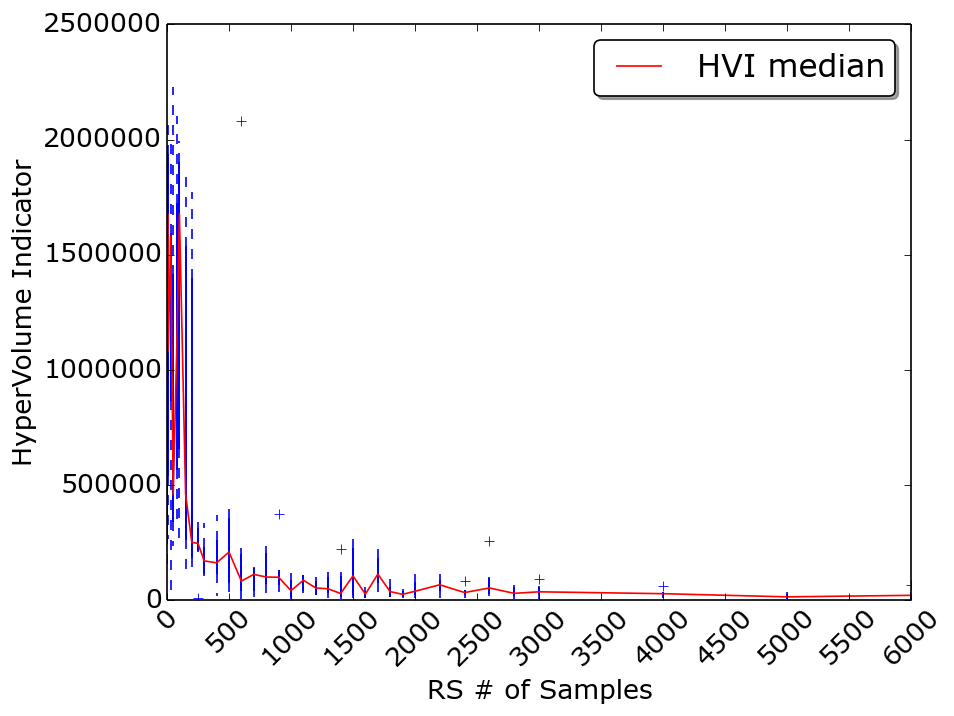
\includegraphics[width=\linewidth]{images/DSE/hvi_5NumberSummary_median.png}
% \subcaption{HyperMapper HVI versus initial random samples ($R$) five number summary.}
% \label{hvi_samples}
% \end{subfigure}\hspace{15pt}
% ~
% \begin{subfigure}[t]{0.45\linewidth}
% 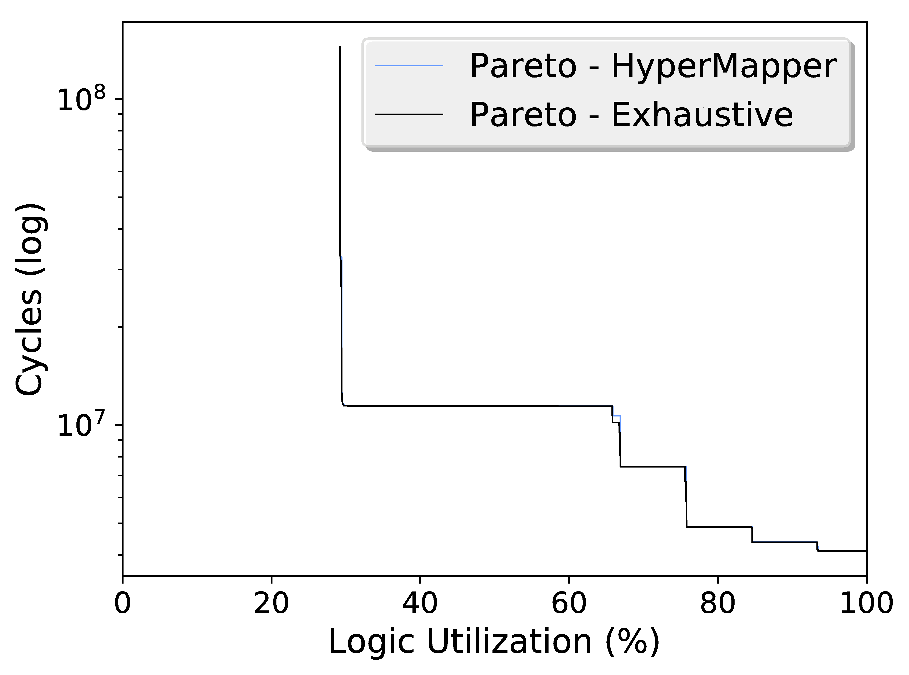
\includegraphics[clip, trim=0.0cm 0.0cm 0.0cm 0.0cm, width=\linewidth]{figs/output_pareto_blackscholes.pdf}
% \subcaption{Exhaustive and HyperMapper ($R$=1000) generated Pareto curves. }
% \label{paretos}
% \end{subfigure}

% \vspace{-10pt}
% \caption{Design space tuning on \emph{BlackScholes}.}
% \label{figHVI}
% \end{figure}

% \begin{table}[ht]
% \centering
% \caption{Runtime to reach accuracy of TODO\% and corresponding variance for design tuning with heuristic search and HyperMapper.\vspace{-10pt}}
% \label{tableDSE}

% \fontsize{7}{9}\selectfont
% \begin{tabular}{llrrrrr}
%                       & \multicolumn{2}{c}{\textbf{Space Size}} & \multicolumn{2}{c}{\textbf{Heuristic}} & \multicolumn{2}{c}{\textbf{HyperMapper}} \\
%                       & \mc{Total} & \mc{Pruned}    & \mc{Time} & \mc{Var}  &   \mc{Time} & \mc{Var} \\ \midrule
%   %\bf{Dot Product}   & 117,964,800      & 1,085,952            &              &                &                &               \\ \midrule  
%   %\bf{Outer Product} & 16,588,800       & 31,068               &              &                &                &               \\ \midrule
%   \bf{BS}             & 7.7$\times 10^4$  & 6.7$\times 10^2$    &              &                &                &               \\ \midrule
%   \bf{GDA}            & 3.0$\times 10^{10}$ & 4.6$\times 10^6$  &              &                &                &               \\ \midrule
%   \bf{GEMM}           & 2.6$\times 10^8$  & 1.4$\times 10^5$   &              &                &                &               \\ \midrule
%   \bf{KMeans}         & 2.1$\times 10^6$  & 1.9$\times 10^4$   &              &                &                &               \\ \midrule
%   \bf{SW}             & 2.1$\times 10^6$  & 3.3$\times 10^4$   &              &                &                &               \\ \midrule
%   \bf{TQ6}            & 3.5$\times 10^9$  & 2.3$\times 10^6$   &              &                &                &               \\ \bottomrule
% \end{tabular}
% \end{table}


\subsection{Spatial Portability}

\begin{table}
\centering
\caption{Runtimes (ms) of tuned designs on ZC706, followed by runtimes and speedup~($\times$) of directly porting these designs to the VU9P, then runtimes and successive speedup over ported designs when tuned for the VU9P. The \emph{Total} column shows the cumulative speedup. \vspace{-5pt} }
\label{fig:zynq_comp}

\centering
\fontsize{7}{9}\selectfont
\begin{tabular}{l d{2.1} d{2.1} d{2.1} d{2.1} d{2.1} d{2.1}}
   \bf{FPGA}      & \mc{ZC706}  & \multicolumn{4}{c}{\bf VU9P}                                       & \mc{Total}     \\ 
   \bf{Design}    & \mc{Tuned}  & \multicolumn{2}{c}{\bf Ported}   & \multicolumn{2}{c}{\bf Tuned}    &               \\ \toprule

                  & \mc{Time}   & \mc{Time}  & \mc{$\times$}       & \mc{Time}  & \mc{$\times$}       & \mc{$\times$} \\ \midrule
   \ml{BS}        & 89.0        & 35.6       & 2.5                 & 3.8        & 9.4                 & 23.4          \\ \midrule
   \ml{GDA}       &  8.4        & 3.4        & 2.5                 & 1.3        & 2.6                 & 6.5           \\ \midrule
   \ml{GEMM}      & 2226.5      & 1832.6     & 1.2                 & 878.5      & 2.1                 & 2.5           \\ \midrule
   \ml{KMeans}    & 358.4       & 143.4      & 2.5                 & 53.3       & 2.7                 & 6.7           \\ \midrule
   \ml{PageRank}  & 1299.5      & 1003.3     & 1.3                 & 587.4      & 1.7                 & 2.2           \\ \midrule
   \ml{SW$^\dag$} & 1.3         &  0.5       & 2.5                 & 0.5        & 1.0                 & 2.5           \\ \midrule
   \ml{TQ6}       & 69.4        & 15.0       & 4.6                 & 14.0       & 1.1                 & 5.0           \\ \bottomrule
   
   \multicolumn{7}{l}{\vspace{10pt}\footnotesize{ $^\dag$SW with 160 base pairs, the largest to fit on the ZC706.}}
\end{tabular}
\vspace{-10pt}
\end{table}

We next demonstrate the portability of Spatial code by targeting two different FPGA architectures; (1) the Zynq ZC706 SoC board, and (2) The Virtex Ultrascale+ VU9P on the Amazon EC2 F1.
Designs on the VU9P use a single DRAM channel with a peak bandwidth of 19.2 GB/s. The ZC706 is much smaller than the VU9P in terms of FPGA resource and has a smaller DRAM bandwidth of 4.26 GB/s.
We target both the ZC706 and VU9P from the same Spatial code for all benchmarks listed in Table~\ref{t:hls_comp}. Benchmarks are tuned for each target using
target-specific models with automated DSE. Clock frequency is fixed at 125 MHz for both FPGAs. 

Table~\ref{fig:zynq_comp} shows the speedups achieved on the VU9P over the ZC706. The results show that not only can the same Spatial source code be ported
to architectures with different capabilities, the application can also be automatically tuned to better take advantage of resources in each target.
Compute-bound benchmarks \emph{BlackScholes}, \emph{GDA}, \emph{GEMM}, \emph{K-Means} achieve speedups of up to $23\times$ on the VU9P over the ZC706. Porting these designs to the VU9P alone has a $1.2\times$ to $2.5\times$ due to increased main memory bandwidth, but a majority of the benefit of the larger FPGA comes from tuning the parallelization factors to use more resources. 
While \emph{SW} is also compute bound, the size of the dataset was limited by the smaller FPGA. In this case, the larger capacity of the VU9P does not improve runtime, but instead allows handling of larger datasets. 

Memory-bound benchmark \emph{TPC-H Q6} benefits from the higher DRAM bandwidth available on the VU9P. Porting this benchmark immediately gives a $4.6\times$ runtime improvement from the larger main memory bandwidth, while further parallelizing controllers to create more parallel address streams to DRAM helps the application make better use of this bandwidth. \emph{PageRank} is also bandwidth-bound, but the primary benefit on the VU9P comes from specializing the memory controller to maximize utilized bandwidth for sparse accesses.


% \begin{table}
% \caption{Speedup of VU9P over ZC706. \vspace{-10pt} }
% \label{fig:zynq_comp}

% \fontsize{8}{10}\selectfont
% \begin{tabular}{cccccc} 
% \bf{GDA}     & \bf{GEMM}    & \bf{K-Means} & \bf{PageRank} & \bf{SW}      & \bf{TQ6} \\ \hline
% 2.54$\times$ & 2.53$\times$ & 1.84$\times$ & 2.21$\times$  & 1.74$\times$ & 4.97$\times$  \\ \hline
% \end{tabular}
% \end{table}




\begin{table}
\centering
\caption{Plasticine DRAM bandwidth, resource utilization, runtime, and speedup ($\times$) over VU9P FPGA. \vspace{-5pt} }
\label{table:plasticine_eval}

\centering
\fontsize{7}{7}\selectfont
\resizebox{0.99\columnwidth}{!}{
  \begin{tabular}{m{0.5cm} d{2.1} d{2.1} d{2.1} d{2.1} d{2.1} d{2.1} r }
  \toprule
                 & \multicolumn{2}{c}{\bf Avg DRAM } & \multicolumn{3}{c}{\bf Resource }        & \mc{}     & \mc{} \\
                 & \multicolumn{2}{c}{\bf BW (\%)}   & \multicolumn{3}{c}{\bf Utilization (\%)} & \mc{Time} & \mc{$\times$} \\
   \bf{App}     & \mc{Load}    & \mc{Store} & \mc{PCU}  & \mc{PMU}  & \mc{AG}   & \mc{(ms)} & \mc{} \\ \midrule
   \ml{BS}       & 77.4        & 12.9       & \mb{\hspace{1pt}73.4} & 10.9      & 20.6      & 2.33      & 1.6   \\
   \ml{GDA}      & 24.0        & 0.2        & \mb{\hspace{1pt}95.3} & 73.4      & 38.2      & 0.13      & 9.8   \\
   \ml{GEMM}     & 20.5        & 2.1        & \mb{\hspace{1pt}96.8} & 64.1      & 11.7      & 15.98     & 55.0  \\
   \ml{KMeans}   & 8.0         & 0.4        & \mb{\hspace{1pt}89.1} & 57.8      & 17.6      & 8.39      & 6.3   \\
   \ml{TQ6}      & \mb{\hspace{2pt}97.2}   & 0.0        & 29.7      & 37.5      & \mb{70.6} & 8.60      & 1.6   \\

\bottomrule
\end{tabular}}
\vspace{-10pt}
\end{table}


Finally, we demonstrate the portability of Spatial beyond
FPGA architectures by extending the compiler to map
the Spatial IR to target our proposed Plasticine CGRA~\cite{plasticine}. Plasticine is a
two-dimensional array of compute (PCUs) and memory
(PMUs) tiles with a statically configurable interconnect
and address generators (AG) at the periphery to perform
DRAM accesses. The Plasticine architecture is a significant departure
from an FPGA, with more constraints on memory banking and computation, including
fixed size, pipelined SIMD lanes.

We simulate Plasticine with  a $16 \times 8$ array of 64 compute and 64 memory tiles, with a 1 GHz clock and a main memory with a DDR3-1600 channel with 12.8 GB/s peak bandwidth.
Table~\ref{table:plasticine_eval} shows the DRAM bandwidth, resource utilization, runtime, and speedup of the Plasticine CGRA over the VU9P for a subset of benchmarks.

Streaming, bandwidth-bound applications like \emph{TPC-H Q6} efficiently exploit about 97\% of the available DRAM bandwidth.
Compute-bound applications \emph{GDA}, \emph{GEMM}, and \emph{K-Means} use around 90\% of Plasticine's compute tiles.
Plasticine's higher on-chip bandwidth also allows these applications to better utilize the compute resources, giving these applications speedups of $9.9\times$, $55.0\times$, and $6.3\times$.
Similarly, the deep compute pipeline in \emph{BlackScholes} occupies 73.4\% of compute resources after being split across multiple tiles, 
giving a speedup of $1.6\times$. 

%We implemented comparable versions of each of our benchmarks in C++ and synthesized them
%using HLS and SDAccel tools.  There are certain constructs in Spatial that allow
%certain algorithms to be expressed more concisely and in slightly different, but intuitive, ways that
%expose the strengths of the language.  Each application exhibits certain characteristics which 
%can be exploited by certain aspects in the programming paradigms of Spatial and HLS. Specifically,
%they can be characterized as compute-bound applications and memory-bound applications, with some
%tradeoff between the two depending on design decisions.  While HLS is the industry standard for
%exposing FPGAs to domain experts, our results show that Spatial is a suitable alternative that can
%lead to better designs for certain algorithms with less overhead.

%Spatial is a suitable platform for the designer who is interested in making the most of the
%available resources, as it allows quick design tradeoffs in the app without needing to use complex pragmas throughout the app.
%In applications that are memory bound, such as AES, BlackScholes, and Sobel, we would expect that neither
%design could acheive significantly better speedup since they have access to the same DRAM interfaces.  
%For compute-bound applications, such as Kmeans, GEMM, and GDA, there is a large, interesting design space that
%Spatial can quickly expose to the user.

%\begin{figure}
%\centering
%\includegraphics[width=1\columnwidth, trim=0.5cm 0.9cm 1.0cm 0]{figs/f1_comp.png}
%\caption{Speedup and resource utilization comparisons with SDAccel on F1.}
%\label{fig:f1_comp}
%\end{figure}

% \subsection{Portability Across FPGAs and CGRAs}
% We demonstrate the applicability of Spatial to beyond FPGA architectures by extending the compiler
% to map Spatial IR to the Plasticine CGRA~\cite{plasticine}. Plasticine is a two-dimensional array of compute (PCUs) and memory (PMUs) tiles
% with a statically configurable interconnect and address generators (AG) at the periphery to perform DRAM accesses.
% Plasticine is a significant departure from FPGA with different kinds of constraints on memory banking and parallelization.

% Similar to the FPGA, we construct area and runtime models specific to Plasticine, and drive the design space exploration to tune
% benchmarks to Plasticine. Compiling to Plasticine then involves lowering the Spatial IR to a target-specific IR for the Plasticine low-level mapping compiler,
% which outputs a configuration bitstream. Resource utilization reports are obtained from the low-level compiler.
% Execution times are measured by simulating the generated bitstream in a cycle-accurate fashion at a clock frequency of 1 GHz. 



%Fortunately, due to the locality exhibited by these applications, designs with large tile sizes that do not maximize the off-chip
%bandwidth are capable of achieving comparable performance to the ones that have 100\%
%compute unit utilization. Hence, the best performing design point shown in
%Table~\ref{table:plasticine_eval} does not correspond to the design with 100\% compute utilization.

%Therefore, the given architecture cannot fit unrolling the outer loop by more than 1 without 
%exceeding 100\% PCU utilization. 
%\todo{K-Means is a sequential iterative convergence algorithm that neither outer loop nor
%inner loop that computes the new centroids can be parallelized.} As a result, we could not maximize
%either bandwidth or resource.}

%For application that are not memory-bound, yet Plasticine is not able to take larger
%unrolling factors, such as BlackScholes and K-Means, Plasticine still achieves roughly $4-7\times$
%speedup compared to F1 due to its higher clock frequency.

%Figure~\ref{fig:gemm_dse} shows the design space of GEMM on Plasticine. The bottom edged circles are
%designs with large tile size that better capture locality. The dark large circles on the right are 
%designs with good PCU and PMU utilization, and high DRAM load bandwidth as result of outer loop
%unrolling. 



%\begin{figure}
%\centering
%\includegraphics[width=1\columnwidth]{figs/GEMM_Blocked.png}
%\caption{Design space for GEMM on Plasticine}
%\label{fig:gemm_dse}
%\end{figure}

%\begin{figure}
%\centering
%\begin{minipage}{.5\linewidth}
  %\centering
  %\includegraphics[width=1\linewidth]{reg_K-FOLD}
  %\caption{Regularization}
  %\label{fig:reg}
%\end{minipage}%
%\end{figure}
%\subsection{GEMM Case Study}
%\gist{gemm}
